%%%%%%%%%%%%%%%%%%%%%%%%%%%%%%%%%%%%%%%%%%%%%%%%%%%%%%%%%%%%%%%%%%%%%%
%% IMPORTANT INFORMATIOn
%% Lines followed by "%% DO NOT CHANGE OR REMOVE" are 
%% system critical, tampering will lead to one or more error messages
%%
%% Lines followed by "%% REQUIRED" contains options that the user 
%% should provide
%%
%% Some lines are followed by "%% OPTIONAL", 
%% and may be omitted (deleted or commented out)
%% 
%% Read the "How To" chapter, 
%% there you will find a detailed explanation of how to use this template, 
%% including examples of all you need and more.
%% 
%%%%%%%%%%%%%%%%%%%%%%%%%%%%%%%%%%%%%%%%%%%%%%%%%%%%%%%%%%%%%%%%%%%%%%

%%%%%%%%%%%%%%%%%%%%%%%%%%%%%%%%%%%%%%%%%%%%%%%%%%%%%%%%%%%%%%%%%%%%%%
%% START PREAMBLE
%% Setting class options,
%% language, metadata, bibliography file, citation style, and more
%%%%%%%%%%%%%%%%%%%%%%%%%%%%%%%%%%%%%%%%%%%%%%%%%%%%%%%%%%%%%%%%%%%%%%


\documentclass[     %% DO NOT CHANGE OR REMOVE
%draft,             %% Turns of graphics rendering and micro-formatting stuff, and turns on todo notes. Affects page breaking. 
cover,              %% Custom cover page, must be provided as an Layout/coverpage.pdf in A4 size- Otherwise a standard HiØ (Høgskolen i Østfold) cover is generated. Default: HiØ standard thesis titlepage
%word,              %% Word-like paragraph formatting, no indentations, air between paragraphs, ragged right. Default: As all documents are formatted, except those made with default M$ documents
%sans               %% Standard HiØ font: Source Sans Pro. Default: Computer Modern, designed by Donald Knuth.
]{thesistemplate}   %% DO NOT CHANGE OR REMOVE


\setdefaultlanguage %% DO NOT CHANGE OR REMOVE
%[variant=bokmal]    %% OPTIONAL. Some languages have variant option, like bokmål and nynorsk for norwegian
{english}         %% REQUIRED. Substitute  with your preferred language (some languages have options), see https://ctan.uib.no/macros/unicodetex/latex/polyglossia/polyglossia.pdf page 6 for supported languages.


%% Metadata, to appear on the half-title page (and the coverpage, if not a custom cover is provided), to be changed by you:

\doctype{Generic Thesis Template}           %% REQUIRED
\department{School of Computer Sciences}    %% REQUIRED
\affiliation{Østfold University College}    %% REQUIRED
\place{Halden}                              %% REQUIRED
\title{The Perfect Thesis}                  %% REQUIRED
\subtitle{Structure, Content and Layout}    %% REQUIRED
\author{Gunnar Misund}                      %% REQUIRED

%% Bibliography and citation style

\citationstyle{ieee} %% REQUIRED. Citation style, see https://www.overleaf.com/learn/latex/biblatex_citation_styles for all available styles, some examples: ieee, apa, nature.
\addbibresource{Bibliography/thesis.bib} %% REQUIRED. You may substitute "thesis" with another. To include more *.bib files, repeat the \addbibresource command

\RequirePackage[toc]{glossaries}
\makeglossaries

\newglossaryentry{latex}
{
    name=\LaTeX,
    description={A mark up language specially suited 
    for scientific documents.\LaTeX\ was developed by Leslie Lamport in 1984, and is basically a collection of macros written in \TeX, invented by Donald Knuth, one of the giants of computer science}
}

\newglossaryentry{maths}
{
    name=Mathematics,
    description={Mathematics is what mathematicians do}
}




    %% OPTIONAL, goes with \printglossaries in the end matter file

%%%%%%%%%%%%%%%%%%%%%%%%%%%%%%%%%%%%%%%%%%%%%%%%%%%%%%%%%%%%%%%%%%%%%%
%% END PREAMBLE
%%%%%%%%%%%%%%%%%%%%%%%%%%%%%%%%%%%%%%%%%%%%%%%%%%%%%%%%%%%%%%%%%%%%%%


%%%%%%%%%%%%%%%%%%%%%%%%%%%%%%%%%%%%%%%%%%%%%%%%%%%%%%%%%%%%%%%%%%%%%%
%% The contents of the rest of the document, 
%% distributed in separate files for chapters and other main parts
%%%%%%%%%%%%%%%%%%%%%%%%%%%%%%%%%%%%%%%%%%%%%%%%%%%%%%%%%%%%%%%%%%%%%%      

\begin{document}

\maketitle          %% DO NOT CHANGE 
\makehalftitle      %% DO NOT CHANGE 
\frontmatter        %% DO NOT CHANGE. Layout of all stuff before Introduction.

\chapter*{About this template}
\addcontentsline{toc}{chapter}{About this template} % DO NOT CHANGE 
\label{chap:about}

This document, along with the source code, is meant to be a self-explanatory generic thesis template, to be used in any field. It is implemented in \LaTeX, the most popular, advanced, flexible, and comprehensive documentation system in natural sciences. However, the document as such could be implemented with other tools, as well.

The thesis covers both structure, content, and layout. No prior \LaTeX\ knowledge is required, since much emphasis has been put on making it user friendly and fairly tampering proof.

The suggested structure is based on the widely used IMRAD model (Introduction, Methods, Results, And Discussion)\footnote{\url{en.wikipedia.org/wiki/IMRAD}}. The student may of course deviate from the structure and recommended content for each chapter. In particular, the chapters describing the main bulk of work done in the research project (Chapters \ref{chap:design}, \ref{chap:implementation}, and \ref{chap:evaluation}), should be customized to fit the specific topic of your project, both regarding chapter titles and content. You may, of course, consider merging some of the chapters, and/or add more chapters.

The template is based on the author's personal experiences as a research scientist and lecturer during the last 25 years\footnote{\url{www.ia.hiof.no/~gunnarmi}}, various online resources, 
and the ``The Mayfield Handbook of Technical and Scientific Writing"  \cite{perelman97mht}\footnote{\url{www.mhhe.com/mayfieldpub/tsw/home.htm}}.

For technical details, see Appendix \ref{chap:how-to}.

For updates and advice regarding this template, and similar templates for Microsoft Word and LibreOffice Writer, follow the Thesis Templates Facebook group\footnote{\url{https://www.facebook.com/groups/693636154649756}}.

Finally: Comments, bug reports, and suggestions are highly welcome\footnote{\url{gunnar.misund@hiof.no}}!

\vspace{20mm}

%\raggedleft
Gunnar Misund

Halden, \today
%\justify





        %%% OPTIONAL 

\chapter*{Abstract}
\addcontentsline{toc}{chapter}{Abstract} % DO NOT CHANGE 
\label{chap:abstract}

An abstract is a brief summarizing statement, not more than one page. It gives the reader a synopsis of the research problem, method, results, and conclusions of your document. The abstract takes the form of a single paragraph and should not contain cross references or citations. Abstracts are sometimes collected into volumes and must be able to stand alone. They may be read by parties trying to decide whether or not to read the main document, or for getting a broad picture before starting on the report. If you describe the content of each main chapter, and bind it nicely together, you’re done. You should not have any information in the abstract that is not found in any of the main chapters. It is common to close the abstract with a few well carefully selected keywords. Obviously, the abstract is the last thing you do in your project. 

Here is an example of a short and concise abstract \cite{winger12e3s}:

\begin{quotation}
\noindent  This thesis presents an evaluation of a set of 3D Scene Graph APIs for Java. The work consists mainly of two parts: Defining a methodology for comparing the APIs, and then applying the proposed methodology to the APIs.
An overview of the available 3D Scene Graph APIs in Java is presented, and a selection of these are chosen for the evaluation. The APIs subjected to the evaluation are Java 3D, Ardor3D and jMonkeyEngine3.
The proposed methodology focuses on the comparison on four different aspects. These are: \textit{Project Management and Technical Infrastructure, System Architecture, System Features and Capabilities, and System Performance}.
The results from applying the evaluation method show that none of the APIs were superior to the others in all respects. The results identify strengths and weaknesses with each API, that indicate which use cases each API might be better suited for.
\newline 
\paragraph{Keywords:} Scene Graph, API, Evaluation, Java, 3D Graphics, OpenGL, Java3D, jMonkeyEngine3, Ardor3D
\end{quotation}




\chapter*{Acknowledgments}
\addcontentsline{toc}{chapter}{Acknowledgments} % DO NOT CHANGE 

In a thesis, it is common to mention the assistance of
people whose help was crucial but not extensive enough to warrant
their being listed as co-authors. Thesis advisors, technicians, and
colleagues  who gave advice or time are all candidates for the
acknowledgments section. Patient family members are also frequently thanked.


\chapter*{Prerequisites (Optional)}
\addcontentsline{toc}{chapter}{Prerequisites (Optional)} % DO NOT CHANGE 
\label{chap:prerequisitest}

You may say something about what kind of knowledge and background the reader should have to get the most from reading your thesis.    %%% OPTIONAL 

\tableofcontents    %% DO NOT CHANGE OR REMOVE
\listoffigures      %% OPTIONAL 
\listoftables       %% OPTIONAL 

%% OPTIONAL. The following is needed if you use code listings
\listingslabel{List of Code} %% Language dependent label used as title of the table of listings
\lstlistoflistings  
\addcontentsline{toc}{chapter}{\thelistingslabel} 
   %% REQUIRED. Contains abstract, acknowledgments, tables of content, etc.
\mainmatter     %% DO NOT CHANGE OR REMOVE. Setting the format and layout for all the stuff from Introduction and on

%% Your chapter files. 
%% This is only a suggestion, you should of course provide chapters and titles that fit your project.

\chapter{Introduction}
\label{chap:intro}

The introduction to your document should lead your
readers into your report and give them an idea of what to expect.
You should
begin with a general statement about the topic before moving on
to specific issues. This strategy will help make the content
accessible to your readers, especially those who are not specialists
in the field. Illustrations, like Figure~\ref{fig:halwin}, often
help to introduce the reader to the problem (from  \parencite{kjeldsen05cor}).

\floatingfigure{Graphics/halden-window}{0.6}{Example of a window query in a map (map from www.finn.no)}
\label{fig:halwin}


In the introduction, you should do the following, in approximately this order:
\begin{compactitem}
  \item State the subject of your document as clearly as possible, and briefly explain why you are doing it (motivation)
    \item Provide necessary and relevant background information (you will elaborate on this matter in Chapter \ref{chap:analysis}, Analysis)
  \item Define the problem you are addressing, your approach to the problem, and why this problem is important
  \item Define the scope of your work (in particular limitations and things you will {\em not} deal with)
  \item Describe your research method, i.e., how you are going to proceed to answer your research question
  \item Give an outline of the rest of the document
\end{compactitem}

You should think of the introduction  as the foundation of your master work, and accordingly you should put considerable efforts in getting it right. 


\section{Background and motivation}
\label{sec:background-motivation}

Here you will describe the topic of your research in broad terms, so that even your grandfather should be able to get the general picture. If you are cooperating with a company, research institute, etc., they should also be introduced. It is also important that you explain {\em why} your topic is interesting and worth researching.

\lipsum[11-14]


\subsection{Research question/Problem statement/Objectives}
\label{sec:research-question}

Every academic paper needs a clearly stated goal, concisely describing its purpose. The formulation depends on the type of document. Here we will see how it can be done in a bachelor’s and master’s thesis. You should put considerable effort in describing your goals, since they will be governing the rest of your work. However, goals may change during the projects, and may need revision now and then.

\paragraph{Bachelor}

A bachelor project is generally more practically oriented than a master’s thesis. Often, the pro-ject has an external project owner, like a company or an institution. The goal will be to provide something that can gain the project owner in some way. Hence, it is important to formulate the effects project owner want to achieve. Objectives often starts with “To\dots”.
The following is from a project developing a social trading app for exchanging used books  \parencite{akeriversen20bah}:

\begin{description}
\item [Objective 1] To connect people that enjoy books with each other.
    \begin{description}
    \item [Objective 1.1] To connect people that enjoy books with each other.
    \item [Objective 1.2] To lessen the environmental effect that printing a new book has.
    \end{description}
\end{description}

If the bachelor project is more theoretically oriented, the goals could be stated as in a master’s thesis, as described in the following section.

\paragraph{Master}

A research question\footnote{It is common with more than one question} is a formal statement of the goal of a study. The research question should clearly and concisely state what the study will investigate or attempt to prove. 
Good research questions help to focus the research and the writing by providing a red thread through the project and the report. 

The research question will surface both in the analysis of the problem, the choice of methods, the design and implementation of the project, and,  most importantly, it will be revisited in the discussion and conclusion parts of the report.

The following example is from  \parencite{killerud14sgs}:

\begin{quotation}
As mentioned, opportunities arise with smart-phones for providing feedback on electricity consumption when coupled with a smart meter. A display such as the eWave, shown in Figure \ref{fig:display}, requires that a user take it upon themselves to check their consumption regularly. An application that notifies the user when consumption is high on a device that, for most parts of the day, is within reach of its owner does not require this initiation. However, it is not certain how such notifications will affect or be perceived by users. Further on in the report I attempt to shed some light on this.
My research question consists of two parts. First, I wish to shed some light on the user experience:


\begin{description}
\item [RQ 1] Given immediate feedback on changes in the electricity consumption through their mobile phone, how do users respond?
\end{description}

Secondly, I wish to see if there is a trend towards a lowering of the electricity consumption peak:

\begin{description}
\item [RQ 2]  What impact does a mobile phone assistant have on electricity consumption patterns in an effect-based billing situation?
\begin{description}
\item [RQ 2.1] You may elaborate in a secondary research question.
\end{description}
\end{description}

\begin{figure}[!htbp]
    \center
    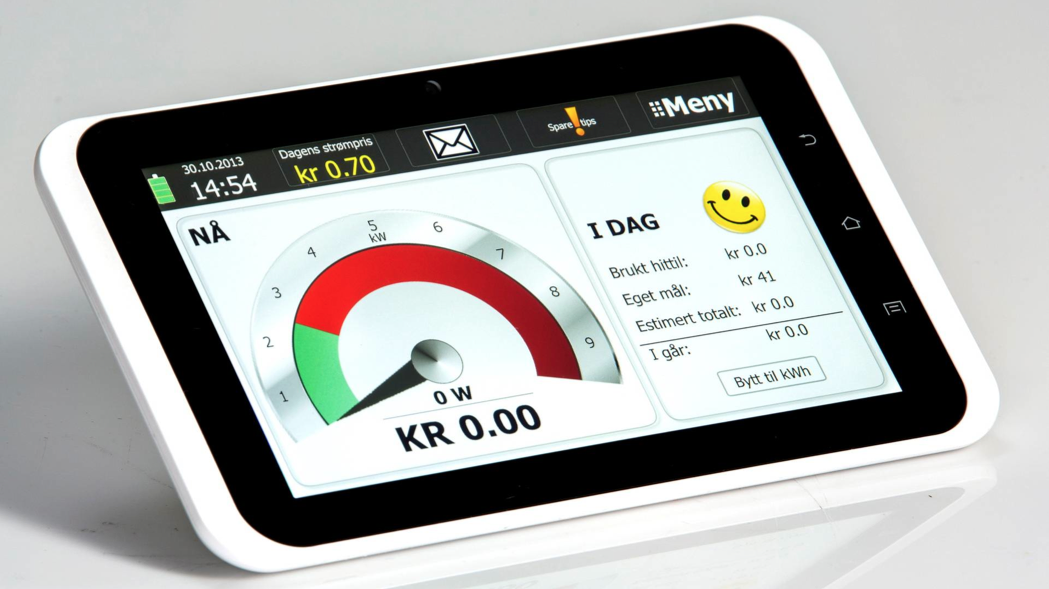
\includegraphics[width=0.6\textwidth]{Graphics/display}
    \caption{The eWave display being offered to Fredrikstad Energi’s customers. The display is 7 inches across, and is based on the Android platform (photo by Odin Media).}
    \label{fig:display}
\end{figure}

\end{quotation}

\subsection{Method}
\label{sec:method}

Here you shall explain how you are going to find answers to the research questions. 
The research method should be treated in more detail later in the report.
Here is an example from  \parencite{nordenhaug11hmf} (it is somewhat sketchy, it is OK to be more detailed than this):

\begin{quotation}
The concept described in this thesis has evolved throughout the work with it, taking on an explorative approach. This process has been incremental using several rounds of iteration before ending
up as a working prototype tested in a real-life setting, involving potential end users throughout the design.
The below mentioned methods have been used in the process:

\begin{compactitem}
\item Identification of research objectives
\item Literature and case studies
\item Development of mock-up videos
\item Implementation of a high-fidelity prototype
\item Field test and interview
\item Testing the prototype on real representative users
\end{compactitem}
\end{quotation}

\subsection{Deliverables}
\label{sec:deliverables}

Here you describe the tangible outcomes of your projects. This obviously includes the thesis, in addition to software, prototypes and such.

\lipsum[7-9]

\section{Report Outline}
\label{sec:outline}

The last point in the introduction is an outline of the rest of the report, for example like this (from  \parencite{kjeldsen05cor}):

\begin{quotation}
Chapter 2 provides background information on range search and line simplification. In the section concerning range search, several data structures and algorithms are presented. The second section describes some of the different techniques developed for performing completely automated line simplification procedures. Finally, another proposed approach to combining the two problems is presented.

The third chapter gives a general description of the PST and what it can be used for. The interval
stabbing problem is an important aspect of the work presented in this thesis, and the third chapter
explains how to solve this with a PST. Next, the interval stabbing problem is expanded to a ``grid
stabbing problem”, which also can be solved using a PST, and the reason for this is described. Chapter 4 gives a detailed description of the new data structure and the search methods that
have been developed. After this, theoretical analyses are provided. This chapter also explains how
an external version of it has been implemented, along with empirical test results to support the theory.

Chapter 5 presents suggestions for further work. Some work on the suggestions that are made has already been conducted, and this work is also described in this chapter. Finally, there is a chapter providing discussions and conclusions to whether or not the problem can be solved using the approach presented in this thesis.
\end{quotation}

      
\chapter{Analysis (Generic title)}
\label{chap:analysis}

This chapter describes the practical and theoretical foundation of your project. Basically, there are two aspects you should focus on, your research topic, and related work (literature and projects).

\section{Research topic (generic title)}

Here you will describe the thesis topic in sufficient detail to work out the details of your project, so that the reader gets a perfectly clear picture of the settings of your project.  It is important to define your scope, and perhaps narrow down a broad subject. Also, if there are such, describe constraints and requirements you need to follow. If your work is part of a larger project, or if you are cooperating with an external company or research institute, this is the place to tell the reader about that.

\lipsum[61-67]

\section{Related work (generic title)}

It is important that you relate your work to relevant research and projects, and base your work solidly on existing literature. 
In particular, you must highlight related work that are directly relevant for your project, for instances if you want to extend earlier research, or to use specific results from other projects.

You should also discuss alternative research methods that have been used to research similar problems.

\lipsum[30-36]

\section{Methods (generic title)}
\lipsum[30-36]

\section{Tools (generic title)}
\lipsum[30-36]

\section{Summary (Optional)}

Sometimes, in particular when the chapters are quite long, they are ended with short summaries.   

\chapter{Design / Planning (Generic title)}
\label{chap:design} 

Here you will explain in detail how you will design you project in order to answer the research question(s). The contents of this chapter will rely heavily on the thesis topic.

 
\lipsum[22-33]
 
\section{Summary (Optional)}






\chapter{Implementation (Generic title)}
\label{chap:implementation} 

This is where you describe what you actually did in your research, like field studies, experiments, implementations, media productions, interviews, etc.



\lipsum[81-99]

\section{Summary (Optional)}
\chapter{Results / Testing / Evaluation (Generic Title)}
\label{chap:evaluation} 

You now present the outcomes of the actual research work described in the previous chapter, as suggested in \parencite{perelman97mht}:


\begin{quotation}
In the results section of a report, describe all appropriate information produced by the research procedures. Simply present data and estimates of their accuracy. Save the explanation and interpretation of these findings for the discussion section, which usually follows the results section. In short documents, however, the results and discussion sections may be combined into a single section.

Results sections make extensive use of graphs and figures to present data effectively. Order information by its importance to your audience's purpose in reading the document. State all significant findings in the text, referring to tables and graphs displaying all significant data. If the study has produced a large amount of raw data, do not present all of it in the results section. Instead, present only the information most appropriate to your audience's purpose in reading the document, summarizing other key information in graphs and figures. If appropriate, include your raw data in an appendix, referring to them within your text.
\end{quotation}

\lipsum[52-60]

\section{Summary (Optional)}




\chapter{Discussion}
\label{chap:discussion} 

You will now discuss and reflect over the results and findings described in the previous chapter. Were they as you expected? How are your findings compared to relevant research? What is the significance of your results? What do you think is your main contribution to the research field? Have your research questions been fully answered? Was it a good choice of research method? Is there anything you would have done differently, in retrospect?

\section{Summary (Optional)}

\lipsum[62-73]






\chapter{Conclusion}
\label{chap:conclusion} 

Some readers of documents, particularly managers, will sometimes not read the entire document but, instead, focus on the conclusion. Hence, this part of the report should summarize all essential information necessary for your audience's purpose. 

In some sense the conclusion is a summary of the discussion chapter. You must relate your findings to the research questions stated in the  introduction, in other words, present the short version of the answer to the research question.
You should also summarize clearly what the report does and does not demonstrate, and what you think is your main contribution to scientific community.

Finally, it is often appropriate to include specific recommendations for future research. Sometimes these recommendations will constitute a separate section.

The conclusion should be relatively short, a page or two is fine.


\lipsum[81-87]



\printbibliography[heading=bibintoc] %% DO NOT CHANGE OR REMOVE. Generates the bibliography from the citations in the text    %% REQUIRED. The main content from Introduction to bibliography
\printglossaries            %% OPTIONAL, goes with the command \RequirePackage[toc]{glossaries}
\makeglossaries

\newglossaryentry{latex}
{
    name=\LaTeX,
    description={A mark up language specially suited 
    for scientific documents.\LaTeX\ was developed by Leslie Lamport in 1984, and is basically a collection of macros written in \TeX, invented by Donald Knuth, one of the giants of computer science}
}

\newglossaryentry{maths}
{
    name=Mathematics,
    description={Mathematics is what mathematicians do}
}




 (before mainmatter.tex)

\appendix                   %% OPTIONAL. Use if you want to include appendices. The following chapters wil be formatted separately as appendices
\chapter{How to use this template}
\label{chap:how-to} 

This document is a generic thesis template covering both structure, content, and layout, to be used as a starting point for bachelor's, master's, and PhD theses in any field. 
It is implemented in the \gls{latex} typesetting markup language, which in particular is suitable 
for documents including \gls{maths} 
and scientific notation, and is considered the gold standard in natural sciences, however commonly used in other settings.

The template is implemented as a document class, 
\texttt{thesistemplate}, with the following options:

\begin{compactdesc}
\item [\texttt{draft}] Turns off graphics rendering and micro-formatting stuff, and turns on todo notes. Affects page breaking.
\item [\texttt{cover}] Custom cover page, must be provided as an Layout/coverpage.PDF in A4 size. Otherwise a standard HiØ (Høgskolen i Østfold) cover is generated.
\item [\texttt{word}] Word-like paragraph formatting, no indentations, air between paragraphs, and ragged right margin. Otherwise standard \LaTeX\ paragraph formatting (as you also find it in most books, papers, and formal documents).
\item [\texttt{sans}] Sans serif fonts, otherwise standard \LaTeX\ font (Computer Modern).
\end{compactdesc}

First of all, it outlines a recommended structure of the thesis, and provides guidelines for the content of each part.
In addition, it serves as a concrete example of how this can be accomplished by using \LaTeX. Use the template by gradually populating the files with your own content, and perhaps modify the structure to suit your project. The template is designed to be rather self-explanatory, and all of the features you need are present somewhere in the source code, so you will come a long way by cutting and pasting.

It is assumed that the user has (or provides herself with) some basic knowledge of \LaTeX. There are numerous good tutorials online\footnote{\url{latex-project.org} is a good starting point}, but I warmly recommend the original documentation: ``\LaTeX: A Document Preparation System'' (Figure \ref{fig:lamport})  \parencite{lamport94ldp}. \LaTeX\ is basically a collection of macros written in \TeX.
This system, which is a low level tool for digital typesetting, is known for producing scientific documents of unprecedented quality. It was developed by Donald Knuth, one of the giants in computer science.

\begin{figure}[!htbp]
\centering 
    
\includegraphics[width=0.3\textwidth]{Graphics/lamport}
    \caption{The \LaTeX\ ``bible'', 2. edition \label{fig:lamport}}
\end{figure}


The template is intended to use with Overleaf\footnote{\url{overleaf.com}}, where it works out of the box.

However, it can be used locally on your machine, using one of the many good \LaTeX\ editors, and there are many possibilities for the Emacs users\footnote{\url{www.gnu.org/software/emacs}}. Personally, I use {\em texmaker}\footnote{\url{www.xm1math.net/texmaker/}}
for OSX, and 
{\em Kile}\footnote{\url{kile.sourceforge.net}}
for Ubuntu. MS users may try {\em WinEDT}\footnote{\url{www.winedt.com}}.


\section{Language settings}

The template is using the \texttt{polyglossia} package, for enabling easy use of different languages, including native UTF-8 support. You may make multi-language documents \footnote{\url{www.overleaf.com/learn/latex/Multilingual_typesetting_on_Overleaf_using_polyglossia_and_fontspec}}. You set the main language for instance like this (in the preamble, before \verb|\begin{document}|):

\verb|\setdefaultlanguage[variant=bokmal]{norwegian}|

See \parencite[p.~6]{polyglossia}\footnote{\url{https://ctan.uib.no/macros/unicodetex/latex/polyglossia/polyglossia.pdf}} for supported languages, including variants.

\section{Chapters/Sections/Paragraphs/Footnotes/Endnotes}

As any document, the template is a collection of chapters, sections, subsections, subsubsections and paragraphs. By default subsubsections and paragraphs are not numbered or included in the table of contents. 

These structural parts contain
plain text and/or graphical elements like figures and tables. 
Plain text is commonly structured by {\em paragraphs}. Paragraphs are generated by one or more {\em empty lines}\footnote{Correspondingly, when there are two or more       consecutive          whitespaces in the text, these will treated as one single whitespace.}. 

{\em Chapters} have {\em sections}, which may contain {\em subsections}, and the next level is {\em subsubsection}.
Finally we have a special type of {\em paragraph}.

Please note that it is considered good practice to have some text before you go to a lower section level, for instance, do not go directly from a chapter to a section, and, in general, do not skip levels, like going from a section to a subsubsection.

Below follows examples of all these constructs.


\section{Section} 
This is a section. \lipsum[10-12]
\subsection{Sub section} 
This is a sub section. \lipsum[13-14]
\subsubsection{Sub sub section} 
This is a sub sub section. \lipsum[15-16]
\paragraph{Paragraph} 
This is a titled paragraph.
Please note the difference between the standard paragraphs produced by blank lines, and this type, which is the lowest level of elements with titles.

{\em Footnotes} are made with the command \verb|\footnote{This is a footnote}|, generating a footnote at the bottom of the page\footnote{This is a footnote}.

In some disciplines, like social sciences, it is common to place the notes in a separate chapter/section at the end of the document. Such notes are called {\em endnotes}, and are made with \verb|\endnote{The end}|\endnote{Definition of an endnote from Merriam-Webster: \say{A note placed at the end of the text}.}. 

\lipsum[17-18]

\section{Figures, tables, equations, etc.}

Please see the source code (\texttt{how-to.tex}) for details on the implementation of these elements.

In general, figures and tables shall be numbered, and have a caption. Numbered figures and tables {\em must} be referenced at least once in the text. Equations and similar elements should also be numbered, but they are not always referred to.

Figures, tables, equations, and similar constructs are so-called {\em floats}. This means that \LaTeX\ will place them in a position that is ``best'', taking many aspects into consideration. The result is that the elements may not be positioned exactly where the author wants (in particular when you have many floats near each other, like in text you are reading now), and novice user may find this frustrating (see Section \ref{sec:bestpractise}). Remember to include empty lines in the source before and after a float.

\begin{figure}[!htbp]
  \begin{center}
    \subfigure[input]{\label{fig:aust}
\includegraphics[width=2.5in]{Graphics/introaustralia}}
    \subfigure[output]{\label{fig:approx}
\includegraphics[width=2.25in]{Graphics/australia_approx}}
  \end{center}
  \caption{Input and result from running the Douglas-Peucker line simplification algorithm (from  \parencite{kjeldsen05cor})}
  \label{fig:dpaustralia}
\end{figure}

Figures are most often produced from files in common graphics formats (like PDF, png, jpg, etc). You can use a single image file, as in Figure \ref{fig:lamport}, or you can combine several images, see Figure \ref{fig:dpaustralia}, consisting of Figures \ref{fig:aust} and \ref{fig:approx}.

The template provides two short-hand commands for including graphics. Figure \ref{fig:floatingfigure} is produced with the \texttt{floatingfigure} command, which let \LaTeX\ to treat it like a floating object, placing it at at the ``best" location. The first argument is the filename, the second gives the width as a fraction of the text width, and the last sets the caption.

\floatingfigure{Graphics/introaustralia}{0.6}{A figure produced by the \texttt{floatingfigure} command}
\label{fig:floatingfigure}

Despite of beeing typed directly after the floating figure, note that this text may for example appear prior to the figure in the PDF.

Ut lectus lectus, ultricies sit amet, semper eget, laoreet non, ante. Proin at massa quisnunc rhoncus mattis. Aliquam lorem. Curabitur pharetra dui at neque. Aliquam eu tellus. Aenean tempus, felis vitae vulputate iaculis, est dolor faucibus urna, in viverra wisi nequenon risus. Fusce vel dolor nec sapien pretium nonummy. Integer faucibus massa ac nullaornare venenatis. Nulla quis sapien. Sed tortor. Phasellus eget mi. Cras nunc.

The \texttt{fixedfigure} command forces the graphics to be placed exactly where it is located in the text
\footnote{Be careful, this could cause some strange effects.}, 
as in Figure \ref{fig:fixedfigure}.

\fixedfigure{Graphics/introaustralia}{0.6}{A figure produced by the \texttt{fixedfigure} command}
\label{fig:fixedfigure}

After inserting a fixed figure, this text should appear directly after the figure in the PDF.

Ut lectus lectus, ultricies sit amet, semper eget, laoreet non, ante. Proin at massa quisnunc rhoncus mattis. Aliquam lorem. Curabitur pharetra dui at neque. Aliquam eu tellus. Aenean tempus, felis vitae vulputate iaculis, est dolor faucibus urna, in viverra wisi nequenon risus. Fusce vel dolor nec sapien pretium nonummy. Integer faucibus massa ac nullaornare venenatis. Nulla quis sapien. Sed tortor. Phasellus eget mi. Cras nunc.

Ut lectus lectus, ultricies sit amet, semper eget, laoreet non, ante. Proin at massa quisnunc rhoncus mattis. Aliquam lorem. Curabitur pharetra dui at neque. Aliquam eu tellus. Aenean tempus, felis vitae vulputate iaculis, est dolor faucibus urna, in viverra wisi nequenon risus. Fusce vel dolor nec sapien pretium nonummy. Integer faucibus massa ac nullaornare venenatis. Nulla quis sapien. Sed tortor. Phasellus eget mi. Cras nunc.

Ut lectus lectus, ultricies sit amet, semper eget, laoreet non, ante. Proin at massa quisnunc rhoncus mattis. Aliquam lorem. Curabitur pharetra dui at neque. Aliquam eu tellus. Aenean tempus, felis vitae vulputate iaculis, est dolor faucibus urna, in viverra wisi nequenon risus. Fusce vel dolor nec sapien pretium nonummy. Integer faucibus massa ac nullaornare venenatis. Nulla quis sapien. Sed tortor. Phasellus eget mi. Cras nunc.
Ut lectus lectus, ultricies sit amet, semper eget, laoreet non, ante. Proin at massa quisnunc rhoncus mattis. Aliquam lorem. Curabitur pharetra dui at neque. Aliquam eu tellus. Aenean tempus, felis vitae vulputate iaculis, est dolor faucibus urna, in viverra wisi nequenon risus. Fusce vel dolor nec sapien pretium nonummy. Integer faucibus massa ac nullaornare venenatis. Nulla quis sapien. Sed tortor. Phasellus eget mi. Cras nunc.

If you want to wrap text around an illustration, the \texttt{wrapfig} package can be used
\footnote{The environment should be placed so as to not run over a page break, that could cause that the figure overlaps the text.}
, as demonstrated in Figures \ref{fig:wrap-inner} and \ref{fig:wrap-outer}.

\begin{wrapfigure}{O}{0.4\textwidth}
  \centering 
  
\includegraphics[width=0.38\textwidth]{Graphics/introaustralia}
  \caption{Wrapped figure placed near the outer margin}
  \label{fig:wrap-outer}
\end{wrapfigure}

Ut lectus lectus, ultricies sit amet, semper eget, laoreet non, ante. Proin at massa quisnunc rhoncus mattis. Aliquam lorem. Curabitur pharetra dui at neque. Aliquam eu tellus. Aenean tempus, felis vitae vulputate iaculis, est dolor faucibus urna, in viverra wisi nequenon risus. Fusce vel dolor nec sapien pretium nonummy. Integer faucibus massa ac nullaornare venenatis. Nulla quis sapien. Sed tortor. Phasellus eget mi. Cras nunc.

Ut lectus lectus, ultricies sit amet, semper eget, laoreet non, ante. Proin at massa quisnunc rhoncus mattis. Aliquam lorem. Curabitur pharetra dui at neque. Aliquam eu tellus. Aenean tempus, felis vitae vulputate iaculis, est dolor faucibus urna, in viverra wisi nequenon risus. Fusce vel dolor nec sapien pretium nonummy. Integer faucibus massa ac nullaornare venenatis. Nulla quis sapien. Sed tortor. Phasellus eget mi. Cras nunc.

\begin{wrapfigure}{I}{0.4\textwidth}
  \centering 
  
\includegraphics[width=0.38\textwidth]{Graphics/introaustralia}
  \caption{Wrapped figure placed near the inner margin}
  \label{fig:wrap-inner}
\end{wrapfigure}

Aenean tempus, felis vitae vulputate iaculis, est dolor faucibus urna, in viverra wisi nequenon risus. Fusce vel dolor nec sapien pretium nonummy. Integer faucibus massa ac nullaornare venenatis. Nulla quis sapien. Sed tortor. Phasellus eget mi. Cras nunc.

Aenean tempus, felis vitae vulputate iaculis, est dolor faucibus urna, in viverra wisi nequenon risus. Fusce vel dolor nec sapien pretium nonummy. Integer faucibus massa ac nullaornare venenatis. Nulla quis sapien. Sed tortor. Phasellus eget mi. Cras nunc.

Aenean tempus, felis vitae vulputate iaculis, est dolor faucibus urna, in viverra wisi nequenon risus. Fusce vel dolor nec sapien pretium nonummy. Integer faucibus massa ac nullaornare venenatis. Nulla quis sapien. Sed tortor. Phasellus eget mi. Cras nunc.

Tables have a relatively steep learning curve.
Still, simple tables, like Table \ref{tab:simple}, are relatively easy to make.
A more complex example is demonstrated in Table \ref{tab:complex}\footnote{An easy workaround is to generate the table in a spread sheet program, export to an image or PDF file and include as graphics.}.

\begin{table}[!htbp]
\centering
\begin{tabular}{c|c|c}
X &  & \\
\hline
& X & \\
\hline
 &  & X \\
\end{tabular}
\caption{Simple table}
\label{tab:simple}
\end{table}

\begin{table}[!htbp]
\centering
\resizebox{0.6\textwidth}{!}{%
\begin{tabular}{|>{\bfseries}c||p{1.0em}|p{1.0em}|p{1.0em}|p{1.0em} l|}      \hline
\textbf{Combination} &\multicolumn{5}{l|}{\textbf{Included Optional Steps}}\\\cline{2-6}
   & \textbf{1}&\textbf{2}&\textbf{3}&\textbf{4}&\\\hline\hline
 1 & X & & & &    \\\hline
13 &  &  & X & X &\\\hline
14 &  &  &  & X & \\\hline\hline
15 & \multicolumn{4}{l}{Nano Particles Deposited, Not Sintered}&\\\hline
16 & \multicolumn{4}{l}{Only Grinded Wafer 1, No Particles Deposited, Not Sintered}&\\\hline
17 & \multicolumn{4}{l}{Only Grinded Wafer 2, No Particles Deposited, Not Sintered}&\\\hline
\end{tabular}}
\caption{Complex table}
\label{tab:complex}
\end{table}

Within mathematics and natural sciences there is a common belief that \LaTeX\ is unrivaled when it comes to typesetting formulas, equations, and complex specialized notation, as the following examples demonstrate.

You can have inline equations, like this: $ \alpha = \beta \gamma \delta $, or you can typeset them as numbered floats, as in Equation \ref{eq:abc}.
\begin{equation}
  \alpha = \beta \gamma \delta
  \label{eq:abc}
\end{equation}

Equation \ref{eq:mom-inert} is a bit more complicated:

\begin{equation}
  I_{zz} = \int_{-b/2}^{b/2} \int_{-h/2}^{h/2} y^2 dy dx = \frac{b h^3}{12}
  \label{eq:mom-inert}
\end{equation}

There are loads of special characters, like $\approx$, $\pm$,
$\times$, $\div$, $\propto$, $\leq$, $\geq$, $\ll$, $\gg$, $\neq$,
$\nabla$, $\Re$, $\Im$, $\flat$, $\sharp$, $\partial$, $\infty$, and $\heartsuit$.


See the next section for a complete example of a mathematical proof.

\section{Proof of the Area of a Circle Formula}

Here follows a complete proof of a theorem.

\newtheorem{prf}{Theorem}

\begin{prf}
The area of circle with radius $r$ is $\pi r^2$.
\end{prf}

\noindent \textbf{Proof:} The equation of a circle centered at the
origin is

$$
x^2 + y^2 = r^2,
$$

\noindent where $r$ is the radius.  We  write $y$ in terms of the
variable $x$ and the constant $r$:

$$
\frac{x^2}{r^2} + \frac{y^2}{r^2} = 1
$$
$$
\frac{y}{r} = \sqrt{1-\frac{x^2}{r^2}}
$$
$$
y= r\sqrt {1-\frac{x^2}{r^2}}
$$

By symmetry, the area of a circle centered at the origin is four
times the area of the circle between $(0,0)$ and $(r, 0)$ above the
$x$-axis.  We can integrate to find the area ($A$):

$$
A = 4r\int_0^r \sqrt {1-\frac{x^2}{r^2}}\, dx
$$

To evaluate the antiderivative of $\displaystyle\sqrt
{1-\frac{x^2}{r^2}}$, we make the substitutions:

$$
x = r \sin \theta
$$
$$
\theta = \arcsin \frac{x}{r}
$$
$$
dx = r\cos \theta\, d\theta
$$

Thus, our integral becomes:

$$
A=4r\int_0^r \sqrt {1-\frac{x^2}{r^2}}\, dx = 4r\int_0^{\pi/2}
r\sqrt{1-\sin^2 \theta} \cos \theta\, d\theta
$$

 We can use the trigonometric identity $1 - \sin^2 \theta = \cos^2 \theta$:

$$
A=4r\int_0^{\pi/2} r\sqrt{1-\sin^2 \theta} \cos \theta\, d\theta=
4r^2\int_0^{\pi/2} \cos^2 \theta\, d\theta
$$

We then apply $\cos^2 \theta = \frac{1}{2}(1 + \cos 2\theta)$:

\begin{eqnarray*}
4r^2\int_0^{\pi/2} \cos^2 \theta\, d\theta &=& 4r^2\int_0^{\pi/2}  \frac{1}{2}(1 + \cos 2\theta) \,d\theta\\
& = & {2r^2\theta}\Bigg{|}_0^{\pi/2} + 2r^2\int_0^{\pi/2} \cos 2\theta \,d\theta\\
                                  & = & \pi r^2 + 2r^2(\sin2\theta)\Bigg{|}_0^{\pi/2}\\
                                  & = & \pi r^2
\end{eqnarray*}

Thus, the area of a circle with radius $r$ is $\pi r^2$.\hfill$\blacksquare$

\section{Listings and other {\em environments}}

You can apply specialized layout by using  {\em environments}. Environments are constructed like this:

\begin{lstlisting}[float=htpb]
\begin{some-environment}
The text and other contents goes here
\end{some-environment}
\end{lstlisting}

The most common environments are the following three different list types\footnote{Here we are using compact versions of the standard lists, which tend to produce to much ``air''}. First, the bullet list:

\begin{compactitem}
\item First item
\item Second item
\item Third item
\end{compactitem}
Then, the enumerated list:
\begin{compactenum}
\item First item
\item Second item
\item Third item
\end{compactenum}
And finally the decription list:
\begin{compactdesc}
\item [First item] First description \lipsum[5]
\item [Second item] Second description
\item [Third item] Third description
\end{compactdesc}

Needless to say, as anything else in \LaTeX, these lists can be customized to your liking.

\subsection{Custom counters}

If you need to number terms or labels, and the list environments do not provide what you are looking for, you can make your own counter and use it to make a new command or environment. In this example, the technique is used to make a table of software reguirements. 

A new counter is generated like this:

\verb|\newcounter{reqcounter}|

Then, for example, you can make a new command using the counter:

\verb|\newcommand{\req}{\refstepcounter{reqcounter} \textbf{R \thereqcounter }}|

\newcounter{rqcount}
\newcommand{\req}{\refstepcounter{rqcount} \textbf{R\therqcount }}

In Table \ref{tab:requirements}, the command is used to automatically generate the numbered IDs. The IDs are labeled, and can be referenced (for instance, requirement R\ref{req:media}).

\begin{table}[!htbp]
    \begin{center}
        \begin{tabular}{|l|l|l|}
             \hline
             ID & Requirement  & Importance  \\
             \hline \hline
             \req \label{req:register} & Registration of new user based on user input & High \\
             \hline
             \req \label{req:media} & Registration of new user based on existing Facebook or Google account & Medium \\
             \hline
        \end{tabular}
    \end{center}
    \caption{Requirements}
    \label{tab:requirements}
\end{table}


\section{Source code}
\label{sec:sourcecode} 

Large chunks of code should be placed in an appendix, but smaller pieces may be listed in the main part. We here demonstrate two ways of doing this.

In Listing \ref{list:hanoi} we have included code from a separate file.

\lstinputlisting[caption=Recursive solution of Towers of Hanoi,label=list:hanoi, language=Java,float=htpb]{Code/hanoi.java}
\index{Recursion|see{Recursion}}
\index{Towers of Hanoi}

Listing \ref{list:hanoi2} is generated by copying and pasting from the same file.

\begin{lstlisting}[caption=Core of the recursive solution of Towers of Hanoi,label=list:hanoi2,language=Java,float=htpb]
// move n smallest discs from one pole to another, using the temp pole
 public static void hanoi(int n, String from, String temp, String to) {
     if (n == 0) return;
     hanoi(n-1, from, to, temp);
     System.out.println(''Move disc '' +n+ '' from '' +from+ '' to '' +to);
     hanoi(n-1, temp, from, to);
}
\end{lstlisting}

\section{Cross-references and bibliography}

As mentioned earlier, all non-text elements should be numbered, and should be referenced to at least once in the text.
This is what is called {\em cross-referencing}, and is easily accomplished.
First we need to attach a label to the element: \verb|\label{type:name}|. Then we use this label in the reference: \verb|\ref{type:name}|. The reference is only a number, so we usually add the element type as a capitalized prefix, for instance like his: \verb|Figure \ref{fig:lamport}}|, which produces: Figure \ref{fig:lamport}.

When you need a reference to an item in your bibliography (books, articles, web sites etc), you need to use one or more ``database'' files, which are plain texts files with bibliography items formatted according to certain rules. These files have the extension \texttt{.bib}, and must be included in the the preamble in the main file.
An example of a correctly formatted bibliography item is found in \ref{list:BibLaTeX}.

\begin{lstlisting}[caption=BibLaTeX entry,label=list:BibLaTeX,language=Tex,float=!htbp]
 @book{perelman97mht,
 author = {Perelman, Leslie and Barrett, Edward},
 title = {{The Mayfield Handbook of Technical and Scientific Writing}},
 year = {1997},
 edition = {1},
 publisher = {McGraw-Hill, Inc.},
 address = {New York, NY, USA},
} 
\end{lstlisting} 

This format is called {\em BibTeX}, and all the academic search engines, including
 {\em Google Scholar}, export to this format.
When referencing, you use this command: \verb|\parencite{perelman97mht}|
and you get: \parencite{perelman97mht}. If you don't want parentheses, 
use \verb|\cite{perelman97mht}|, which gives you: \cite{perelman97mht}. 
If you need to specify page(s), use \verb|\parencite[p. XX]{perelman97mht}|, which results in \parencite[p. XX]{perelman97mht}.
 
To build the bibliography, use the command \verb|\printbibliography[heading=bibintoc]|, which also places an entry in the table of contents.
BibLaTeX generates the  bibliography only from the references in the document (and not from all the items in the \texttt{.bib} files).

The different scientific communities have their own guidelines for how to format the entries in the bibliography, and how to format the references in the document.
You decide which style to use with the command \verb|\citationstyle{<the_style_name>}| in the preamble in the main files\footnote{For an overview of available styles, see \url{https://www.overleaf.com/learn/latex/Biblatex_citation_styles}}.

There are many options for creating specialized bibliographies, for instance multiple bibliographies\footnote{\url{www.overleaf.com/learn/latex/bibliography_management_with_biblatex}}.

There are several tools for creating and maintaining bibliography databases that export BibLaTeX files, both standalone programs, plugins to editors and browsers, and cloud based services\footnote{For instance, check out \url{zotero.org}}. I recommend to use such reference managers, in particular the online versions which, when shared, enable collaborative writing.

\section{Glossary and Index}

You may also make a glossary page, where the terms have descriptions and lists of pages they occur on. You need to provide the terms and their descriptions in the preamble, for instance in a separate file, see \verb|glossary.tex|. An entry looks like this:

\begin{lstlisting}[float,float=!htbp]
\newglossaryentry{maths}
{
    name=mathematics,
    description={Mathematics is what mathematicians do}
}
\end{lstlisting}

The terms are marked in the text like this:

\verb|\gls{latex}|

which generates
\gls{latex}. The glossary is produced by including \verb|\\printglossaries| in the main file, and run \verb|makeglossaries| when compiling. 

The result in the glossary will be something like this:  

``mathematics Mathematics is what mathematicians do. 1, 29''.

An index is made by marking words, for instance \index{IMRAD}, like this

\verb|\index{IMRAD}|

The index page is then produced by including \verb|\printindex| in the main file, and running the following sequence\footnote{Overleaf does this automatically when compiling.}:

\begin{lstlisting}[float,float=!htbp]
xelatex main
makeindex main
xelatex main
\end{lstlisting}

The entry in the index page will then be:  

``IMRAD, 48''.

\section{Fonts}

For every  \LaTeX\ distribution, there is a default set of fonts.
It is possible to customize this setup.
Normally, there is no need for this.
Nevertheless, to change the fonts for the whole document, use the following command in the preamble:

\verb|\usepackage[lining,light,default]{sourcesanspro}|
with the name of the typeface and the appropriate options\footnote{For a list of available fonts, see for instance \url{www.overleaf.com/learn/latex/font_typefaces\#Reference_guide}}.

However, size, weight, style, and typeface may be manipulated using standard commands.

\paragraph{Font size}

First of all, you decide in the preamble the default font size for your document. The \texttt{documentclass} takes the parameters \texttt{10pt},  \texttt{11pt},  or \texttt{12pt}. Locally, you can change the style by these commands, that resizes the font {\em relatively} to the default size:

    \tiny tiny
    
    \scriptsize scriptsize
    
    \footnotesize footnotesize
    
    \small small
    
    \normalsize Default: normalsize
    
    \large  large
    
    \Large Large
    
    \LARGE LARGE
    
    \huge huge
    
    \Huge  Huge
    
    \normalsize 
    
\paragraph{Font weight (Font series)}
You can locally change the font weight:
    
    \textmd{Default: Medium}
    
    \textbf{Bold}
    
    
\paragraph{Font style (Font shape)}
The font style may also be locally changed:
    
    \textup{Default: Normal (Upright/Roman)}
    
    \textit{Italic}
    
    \textsl{Slanted}
    
    \textsc{Small caps}
    
\paragraph{Font family}
Here is how you locally change font family:
 \begin{compactitem}
  \item \textrm{Default: Roman (serif)}
  \item \textsf{Sans serif}
  \item \textit{Italic}
  \item \textbf{Bold}
  \item \textmd{Medium}
  \item \textsl{Slanted}
  \item \textup{Upright}
  \item \textsc{Small caps}
  \item \textbf{Bold}
 \end{compactitem}   
    
    
\section{To-do notes}
\label{sec:miscellaneous}

Many find it useful to use todo-notes. You can place it inline, with

\verb|\todo[inline]{This is an inline note.}|

\todo[inline]{This is an inline note.}
Or, if you prefer, in the margin with 

\verb|\todo[inline]{This is a margin note.}|

\todo{This is a margin note.} The todo notes will only be visible when using the \texttt{draft} option in the document class.

\section{Compilation}


Making documents with \LaTeX\ is basically like writing software. 
This document is produced by compiling a collection of files, all in the same folder.
There is a top level file called 
\texttt{main.tex}, which contains commands that decide format, layout etc., or in other words, the {\em style}\footnote{Think of HTML and stylesheets \dots guess where that idea came from \dots}. It also includes the files containing the actual text (in general one file for each chapter).

When using Overleaf, the compilation is done automatically when saving a file in the project, or when issuing the \texttt{Recompile} command.


When using the template locally, you may compile it with the appropriate commands in your IDE, or do it from the command line. To generate a PDF file, go to the document folder, and issue the following commands: 

\begin{compactenum}
\item \verb|xelatex main| (runs through the document, setting up various help files and generates a preliminary PDF)
\item \verb|biber main| (generates the bibliography from the citations)
\item \verb|xelatex main| (includes the bibliography)
\item And finally yet another \verb|xelatex main| to get all cross-references and citations correct.
\end{compactenum}


This process produces a PDF file,
\texttt{main.PDF}. When printing this particular document, remember to select the double page option.

\section{Quotes and quotations}

\LaTeX\ is picky on quotation marks, to produce correct start and end marks you should type \verb|``a quote''|, which produces ``a quote''. To be on the safe side, use the \verb|\say| command, which also enables nested quotes, like this: \say{A quotation may have \say{nested} quotations}.

Quotation marks are used when you want inline quotes. However, longer quotations should be made with the ``quote'' (or ``quotation'') environment:
\begin{quote} 
    \lipsum[3-4]
\end{quote}

Remember to always cite the source of a quotation like this.

\subsection{Troubleshooting}

As you may experience when compiling the source code, there might be syntax errors, missing files etc. to be fixed. In Overleaf, error and warning messages are displayed as colored margin markers in the source text, and in the PDF pane. Red flags are indicating errors that Overleaf/\LaTeX\ is not able to fix, thus not able to generate the PDF. These needs to be fixed by you. Overleaf tries to repair minor errors, giving red flags, but still generates the PDF. These errors should also be corrected.

You should also try to fix the orange warnings, but they are not critical. Blue warnings may be ignored, they mostly complain about ``overfull'' and ``underfull'' boxes, which in most cases do not affect the final document in any perceivable way.

If stuck, consult the Overleaf troubleshooting pages\footnote{\url{www.overleaf.com/learn/latex/Errors} and
\url{www.overleaf.com/learn/latex/Questions/Tips_and_Tricks_for_Troubleshooting_LaTeX}}. In some rare cases you need to delete all temporary help files, if so, go to the bottom of the error/warning pane and choose ``Clear cache''. If you run the project locally, this is done by deleting all \texttt{main.*} files, except \texttt{main.tex}.

However, sometimes it can be really tricky to find the source for an error. You should typically search backwards from where the error occurs. Listing \ref{list:latexerror} is an example from compiling this document, where the error is 
misspelling of the \LaTeX\  macro (should be \verb|\LaTeX|, not \verb|\LateX|). The key error message is ``\verb|! Undefined control sequence|'', followed by a quote of the line where the error has occurred, along with the line number. The name of current file is found a couple of lines above: ``\verb|(./how-to.tex|''.

\begin{lstlisting}[float=htpb, caption=\LaTeX\ error output,label=list:latexerror]
...

Overfull \hbox (6.0pt too wide) in paragraph at lines 43--44
[][][][][][]

Underfull \hbox (badness 10000) in paragraph at lines 43--44

) (./conclusion.tex [20]
Chapter 7.
[21]) (./main.bbl [22]) [23] [24]
No file main.ind.
(./how-to.tex
Appendix A.
[25]
! Undefined control sequence.
l.48 misspelling of the  \LateX
                         \  macro (should be \verb|\La...

? 
} 
\end{lstlisting} 



\section{Best practice}
\label{sec:bestpractise}

\begin{compactitem}
\item First: Focus on {\em content} and {\em structure} 
\item Later: Decide on layout and style
\item Use mostly the default settings
\item If you need special functionality, look for packages covering your needs
\item If you do not find suitable packages, make your own macros
\item Learn by 1) asking fellow students, 2) google and cut'n paste, and 3) by sending me an email or come to my office
\item Compile frequently
\item Commit frequently to your versioning system\footnote{SVN is a good choice, or use any of the many free online services.}
\item Run spell checks when things start to get complete\footnote{Most editors provide built-in spell check functionality (which ignores the markup commands).  On Linux platforms you have the ispell and aspell command line tools which can be configured for \LaTeX. There are also stand-alone tools around.}
\item When the document absolutely complete: perform minor fine-tuning (typically to sort out bad placements of floats). Remember that every fix you apply may affect the subsequent layout.
\end{compactitem}



     %% READ THIS CHAPTER: A detailed user manualm, with sample code of everything you need and more :-)

\end{document}              %% DO NOT CHANGE OR REMOVE     %% REQUIRED. Appendices, glossary and such

%%%%%%%%%%%%%%%%%%%%%%%%%%%%%%%%%%%%%%%%%%%%%%%%%%%%%%%%%%%%%%%%%%%%%%
%% END OF MAIN.TEX
%%%%%%%%%%%%%%%%%%%%%%%%%%%%%%%%%%%%%%%%%%%%%%%%%%%%%%%%%%%%%%%%%%%%%%